\section{Schmitt-Trigger}

\begin{itemize}
    \item Schaltschwellen müssen nicht sehr genau sein
    \item Schmitt-Trigger garantieren auch bei verrauschten Signalen saubere (einmalige) Schaltschwellen, dank der Hysterese
\end{itemize}



\subsection{Aufbau nichtinvertierender digitaler Schmitt-Trigger}

\begin{minipage}[position]{0.35\columnwidth}
    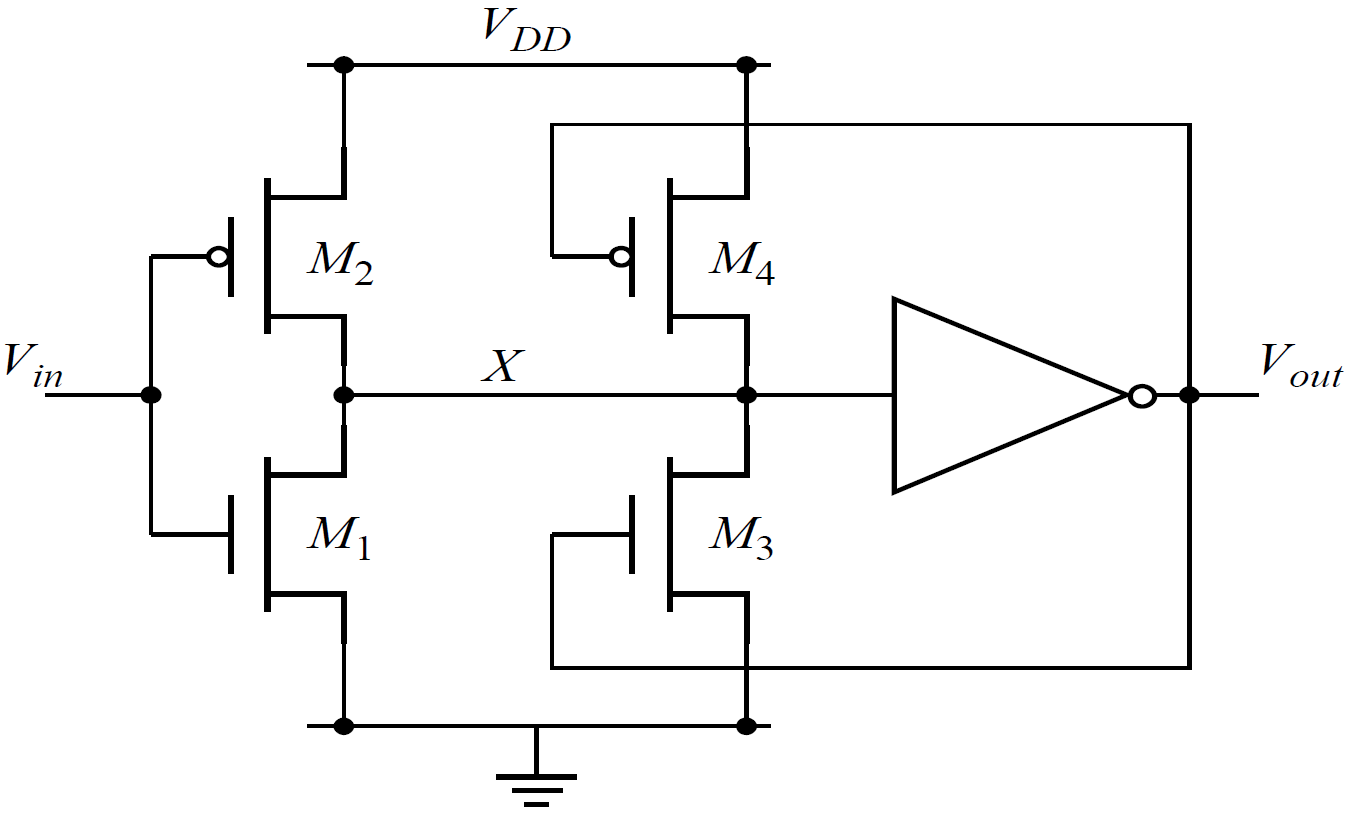
\includegraphics[width=\columnwidth]{images/nichtinvertierender_schmitt-trigger.png}
\end{minipage}
\hfill
\begin{minipage}[position]{0.63\columnwidth}
    \begin{itemize}
        \item $M_1, M_2$: Digitale Inverter
        \item $M_3, M_4$: gesteuerte Widerstände
        \item \textbf{Für }$\boldsymbol{V_{\rm out} = 0}$: $M_4$ leitet, $M_3$ sperrt
        \item \textbf{Für }$\boldsymbol{V_{\rm out} = 1}$: $M_3$ leitet, $M_4$ sperrt
        \item $M_3, M_4$ verschieben Schaltschwellen abhängig von $V_{\rm out}$ \textrightarrow\ Hysterese
    \end{itemize}
\end{minipage}


\subsection{Aufbau invertierender digitaler Schmitt-Trigger}

\begin{minipage}[position]{0.3\columnwidth}
    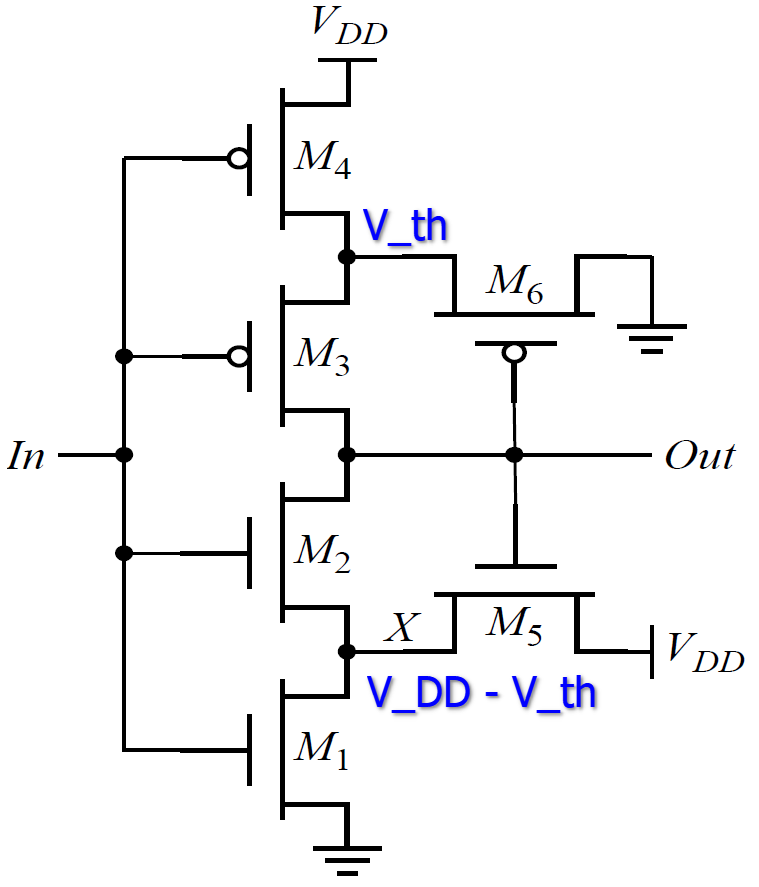
\includegraphics[width=\columnwidth]{images/invertierender_schmitt-trigger.png}
\end{minipage}
\hfill
\begin{minipage}[position]{0.68\columnwidth}
    \begin{itemize}
        \item Ohne $M_5, M_6$: Normaler Inverter mit je 2\\
            Serie-Transistoren
        \item \textbf{Für }$\boldsymbol{V_{\rm out} = 1}$: Durch $M_5$ fliesst Strom in $M_1$
        \item $V_{\rm in}$ muss höher sein, um Strom der PMOS aufzunehmen\\
            \textrightarrow\ Höhere Schaltschwelle für High-Low-Übergang
        \item 'Inverses' gilt für $M_6$ und $M_4$
    \end{itemize}
\end{minipage}


\subsection{Schmitt-Trigger vs. CMOS-Logik}

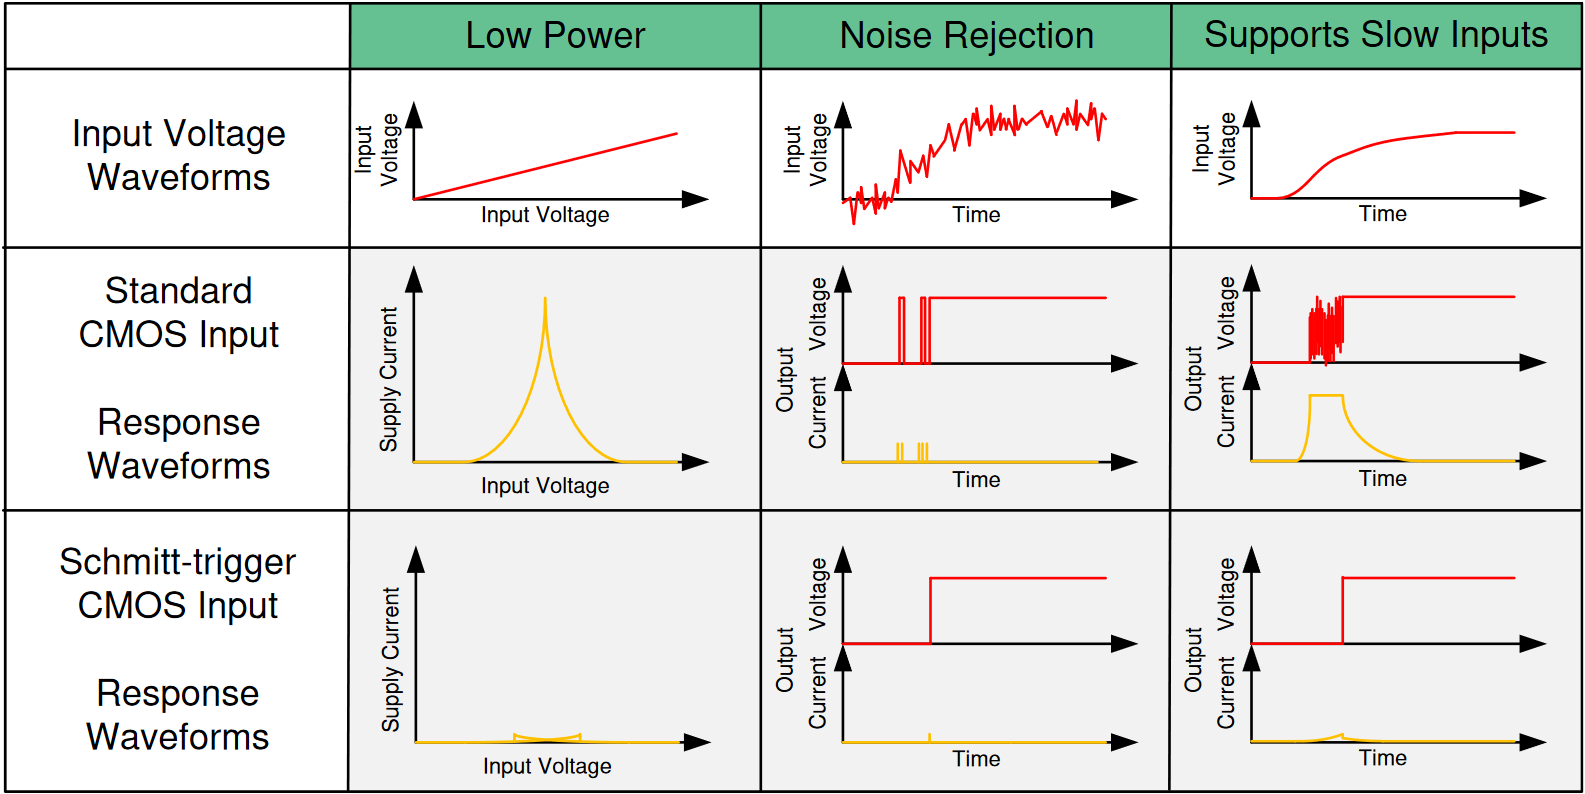
\includegraphics[width=\columnwidth]{images/benefits_schmitt-trigger.png}

